\chapter{Entanglement generation in front of a fixed shield}\label{cha:entanglement-generation}


\begin{figure}[!htbp]
  \centering
  \def\svgwidth{\textwidth}
  \input{./../figures/problem.pdf_tex}
  \caption{My problem}
  \label{fig:4:problem-scetch}
\end{figure}

\begin{figure}[!htbp]
  \centering
  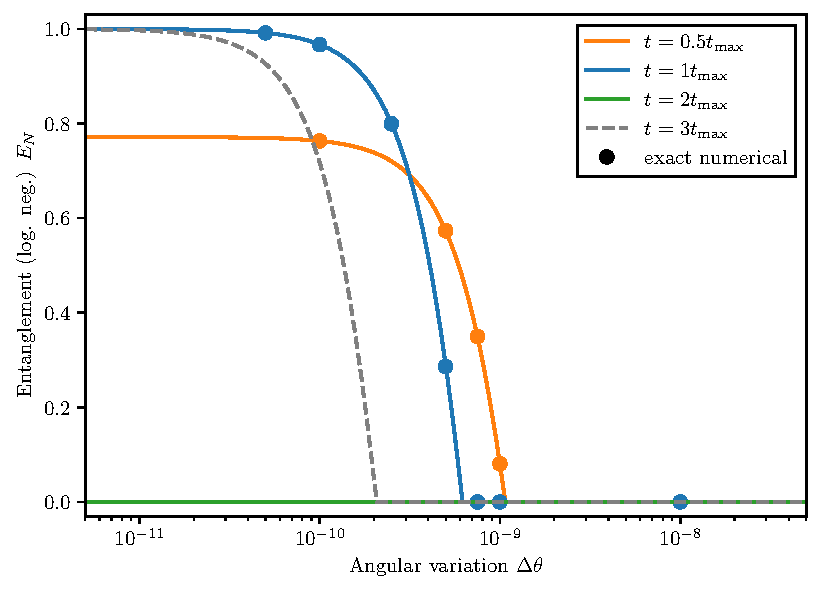
\includegraphics[width=\textwidth]{./../figures/theta-variance/EN-delta-theta.pdf}
  \caption{Entanglement quantified by the logarithmic negativity (eq. \eqref{eq:2:logarithmic-negativity}) dependent on the angular variation $\Delta\theta$. The entanglement is shown at different times, where $t_\mathrm{max}$ is the time of maximal entanglement calculable by eq. \eqref{eq:4:t-max}. Additionally, a few selected exact numerical results are shown to align precisely with the approximated version.}
  \label{fig:4:EN-delta-theta}
\end{figure}


\section{Orientation}
$E_N$ depending on the orientation:

\begin{equation}
  E_N = \log_2\left\{
    1 + \abs{
      \sin(
      \frac{G M_A M_B t}{\hbar} \frac{\Delta x_A \Delta x_B}{8L^3}
      \left[ \sin\alpha\sin\beta - \frac{1}{2}\cos\alpha\cos\beta \right]
      )
      }
  \right\}
\end{equation}

Time till the maximum entanglement ($E_N = 1$):
\begin{equation}\label{eq:4:t-max}
  t_\mathrm{max} = \frac{8 \pi L^3 \hbar}{2 G M_A M_B \Delta x_A\Delta x_B} \abs{\sin\alpha\sin\beta - \frac{1}{2}\cos\alpha\cos\beta}^{-1}
\end{equation}

with a global minimum for $\alpha,\beta \in [0, \pi]$ for the orthogonal orientation with $\alpha = \beta = \pi/2$. Here, the time till the maximum entanglement is given by
\begin{equation}
  t_\mathrm{max} = \frac{4 \pi \hbar L^3}{G M_A M_B \Delta x_A \Delta x_B} \simeq 129\si{mn}
\end{equation}

\begin{figure}[!htbp]
  \centering
  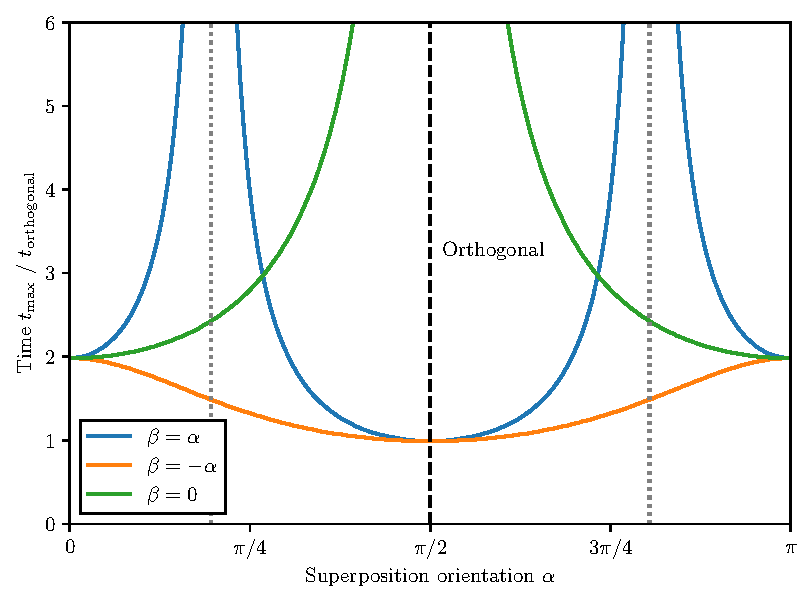
\includegraphics[width=\textwidth]{./../figures/ideal-entanglement/EN-orientation.pdf}
  \caption{Time until maximal entanglement $t_\mathrm{max}$ for different orientations of the angled $\alpha$ and $\beta$ (refer to \cref{fig:4:problem-scetch}). The \textit{parallel configuration} corresponds to $\alpha = \pm\beta = k\pi$ and the \textit{orthogonal configuration} to $\alpha = \pm\beta = k\pi - \pi/2$ ($k \in \mathbb{Z}$). The minimal time is reached for the orthogonal configuration.}
  \label{fig:4:tmax-orientation}
\end{figure}

\begin{figure}[!htbp]
  \centering
  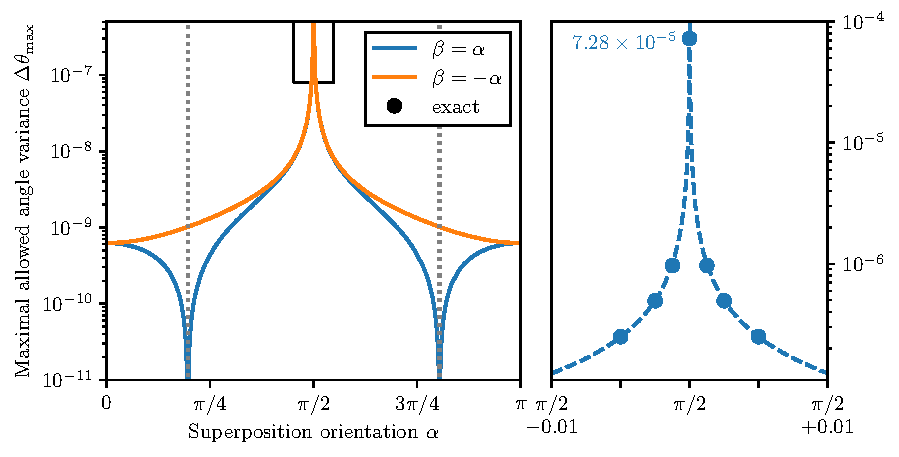
\includegraphics[width=0.95\textwidth]{./../figures/theta-variance/theta-max-orientation-complete.pdf}
  \caption{Maximum possible allowed angular variation $\Delta\theta_\mathrm{max}$ for different orientations. All data-points where calculated at the time of maximum entanglement shown in \cref{fig:4:tmax-orientation}. The \emph{orthogonal configuration} is very stable against angular disturbances. At $\alpha=\beta=\pi/2$, only exact numerical results show a finite value. The singularities on the left figure arise from the fact, that these configurations need infinite time to entangle as already seen in \cref{fig:4:tmax-orientation}.}
  \label{fig:4:theta-max-orientation}
\end{figure}

\begin{figure}[!htbp]
  \centering
  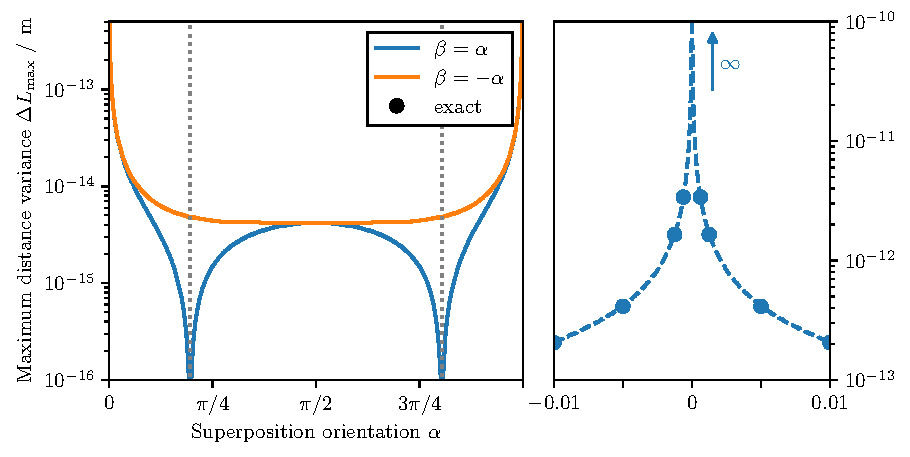
\includegraphics[width=0.95\textwidth]{./../figures/L-variance/L-max-orientation-complete.pdf}
  \caption{Maximum possible allowed distance variation $\Delta L_\mathrm{max}$ for different orientations. This figure is similar to \cref{fig:4:theta-max-orientation}, only for distance variations. On the contrary to angular variations, the \emph{parallel configuration} is infinitely stable against changes in the distance between the shield and the cat-state.}
  \label{fig:4:L-max-orientation}
\end{figure}

\begin{figure}[!htbp]
  \centering
  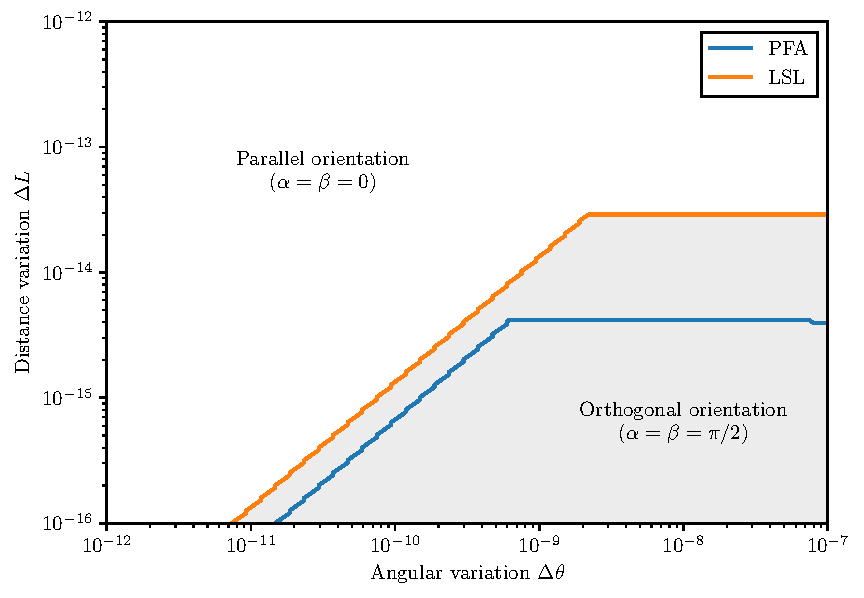
\includegraphics[width=\textwidth]{./../figures/optimize/optimized-orientation.pdf}
  \caption{Optimal orientation for arbitrary variations in the angle $\Delta\theta$ and the distance $\Delta L$. The optimum was calculated for different models of the Casimir-interaction (PFA eq. \eqref{eq:3:casimir-sphere-plate-PFA} and LSL eq. \eqref{eq:3:casimir-sphere-plate-LSL}).If angular variations dominate, the orthogonal configuration is best, whereas for large distance variations, a parallel orientation is advised.}
  \label{fig:4:optimal-orientation}
\end{figure}

\section{Discussions}\label{sec:4:discussion}
The preceding results highlight, that the proposed Faraday shield in experiments on measuring gravitationally induced entanglement entail significant engineering challenges, particularly due to the strict accuracy requirements for particle placement.
Variations must be minimized to a precision of approximately $\Delta L \simeq 10^{-10}\si{m}$ and $\Delta \theta \simeq 10^{-9}\si{rad}$, which are extremely stringent.
Even the rotation of the earth ($\omega_\mathrm{Earth}\approx 7.3\times 10^{-5}\si{rad/s}$) could potentially be problematic, because if small fluctuations in the measurement time $\Delta t \gtrsim 10^{-4}\si{s}$ are present, this corresponds to an additional angular uncertainty of $\omega_\mathrm{Earth}\Delta t \gtrsim \Delta \theta_\mathrm{crit}$.
Adjustments to the experimental parameters in \cref{tab:paramters} have to be made, where especially the separation distance $L$ and the orientation are easily changeable.

The parallel configuration is very stable against variations in the distance and might therefore be favorable (see in \cref{fig:4:optimal-orientation}).
The separation $L$ can be freely chosen and larger distances reduce the effect of placement variations as seen in \cref{fig:4:theta-crit-L}, while simultaneously increasing the required coherence time $t_\mathrm{max} \propto L^3$.

It could also be argued that at a distance of $L \geq 100\si{\mu m} = 10 R$ (compare to \cref{sec:2:experimental-problems}), the Faraday shield would no longer be required because the Casimir forces are approximately ten times weaker than gravitational interactions.
However, the loss of entanglement due to angular and distance variations is not purely due to the Casimir forces between the particle and the shield.
The gravitational coupling also depends on the placement, so that a complete removal of the shield does not fully eliminate the need for high placement accuracy.
Without the shield and by gravitational interaction alone, the critical variations are given by $\Delta \theta_\mathrm{crit,\,ideal} = 1.1 \times 10^{-3}\si{rad}$ and $\Delta L_\mathrm{crit,\,ideal} = 7\times 10^{-4}\si{m}$, which should not pose an engineering problem.

Other parameters, such as particle size and superposition size, may not be easily adjustable without increasing the complexity of quantum control.
Furthermore, particle trapping and levitation is not a limiting factor, as stable trapping is achievable for various configurations (\cref{sec:4:trapping}).

A primary aim of this thesis is to assess whether the Faraday shield allows particles to be brought closer together to enhance gravitational entanglement and reduce coherence times. 
Using the previous results, a optimal experimental parameter space can be determined.
The optimization-goal can be expressed as the following:

One wants to get \textit{as much entanglement as possible} in the \textit{shortest time possible} while allowing for the \textit{largest uncertainties} in the state preparation and considering the limitations in the particles mass as well as in the superposition size.

Without specific constraints, a general optimization is impossible because (if the mass $M$ and the superposition size $\Delta x$ is fixed) coherence time $t \propto L^3$ (eq. \eqref{eq:4:t-max}) and critical angular variation $\Delta \theta_\mathrm{crit} \propto (L-R)^3/L^3$ (for small separations) or $\Delta \theta_\mathrm{crit} \propto L^2$ (for $L \gg R$) cannot be optimized simultaneously.
With constraints such as target coherence time $t_\mathrm{target}$ and/or a minimum placement accuracy, the required sphere-plate separation $L$ as well as maximum measurable entanglement can be determined using the following steps:
\begin{enumerate}
  \item Let us assume that the size of the particle $R$ and consequently the mass $M=4/3 \pi R^3 \rho_\mathrm{Silica}$ as well as the superposition size $\Delta x$ are fixed. An increase in either of them would have a positive effect of the optimization goal stated above, as the time $t_\mathrm{max}$ decreases and the stability against placement variations increases simultaneously.
  \item Given placement accuracies in angular and separation variations determine the optimal orientation $\alpha,\beta$ of the setup as seen in \cref{fig:4:optimal-orientation}. Experimentally reachable coherence times may influence this decision slightly by taking \cref{fig:4:t-max-orientation} into account. Most likely, the most stable orientation is going to be the parallel one with $\alpha = \beta = 0$.
  \item The following ratio given by the entanglement rate eq. \eqref{eq:4:t-max}
  \begin{equation}
    \frac{M^2 (\Delta x)^2}{L^3}t_\mathrm{max} = \frac{4 \pi \hbar}{G}\abs{\sin\alpha\sin\beta-\frac{1}{2}\cos\alpha\cos\beta}^{-1} \sim 10^{-23} \si{kg^2 s/m}
  \end{equation} 
  is fixed therefore \cite{Aspelmeyer_2024}.
  \item In general it is possible to measure at an earlier time $t_\mathrm{target} = \tau t_\mathrm{max}$ (i.e. the coherence time) with $\tau \leq 1$, where less entanglement has been generated but a larger stability against placement variations can be tolerated (see \cref{fig:4:time-delta-theta}). Putting all assumptions together, the product
  \begin{equation}\label{eq:4:fixed-ratio}
    \tau L^3 = \frac{t_\mathrm{target} G M^2 (\Delta x)^2}{8\pi \hbar} = \mathrm{const.}
  \end{equation}
  of measurement time and particle-shield separation is constant.
  \item In the parallel orientation, the distance variations don't matter as the system is very stable against variations in the particle-shield separation. The critical angular variation however scales like $\Delta \theta_\mathrm{crit} \sim (L-R)^3/L^3$ for small distances and like $\Delta \theta_\mathrm{crit} \sim L^2$ at larger distances as shown in \cref{fig:4:theta-crit-L}. It is therefore possible to determine the minimum separation $L_\mathrm{min} > R$ for a given placement accuracy.
  \item Using the required separation, one can calculate $\tau \in (0, 1]$ using eq. \eqref{eq:4:fixed-ratio} and look up the maximal possible entanglement in \cref{fig:4:time-delta-theta} after an evolution time $\tau t_\mathrm{max}$.
\end{enumerate}
As an example, the radius is fixed at $R=10\si{\mu m}$ and the superposition size is $\Delta x = 100\si{nm}$. Let's say that such a particle can be placed with an accuracy of $\Delta \theta = 5 \times 10^{-8} \si{rad}$ and a coherence time of $1\si{s}$ is reachable. 
Using the steps outlined above, the required minimum particle-shield separation is around $L\approx 8R$ and the maximal amount of measurable entanglement is given by $E_N \approx 6.0\times 10^{-2}$.
For more entanglement, either a heavier particle, a larger superposition size, a higher placement accuracy or larger coherence times are required. 
It is therefore possible to bring the particles closer together than without the Faraday shield and still measure entanglement.
One is only limited by the placement accuracy and repeatability.